%version of 11-26-19

\chapter{SOLUTION TO EXERCISES}
\label{ch:Exercises}



\section{Chapter 2. Doing maths -- Proof techniques}

\subsection{A graphical proof}

\noindent \textit{The aim.}

Use a pictural argument to prove a nonobvious identity of arithmetic sums
that one would be unlikely to come upon by purely textual thinking.
\medskip

\noindent \textit{The problem.}
%\label{thm:an-arithmetic-identity}
Prove the following property:

or any positive integer $n$,
\[ \Delta_{2n-1} \ = \ n + 4 \Delta_{n-1}. \]
\medskip

\noindent \textit{The solution.}

Consider the arithmetic series in (\ref{eq:arith-seq}) for the case
$a=1$ and $b=4$.  
By Proposition~\ref{thm:sum-of-arithmetic-series},
this series, call it $S^{(1,4)}(n)$, has the sum
\begin{equation}
\label{eq:triangles}
S^{(1,4)}(n) \ = \ n + 4 \Delta_{n-1}.
\end{equation}

Let us represent the sum $\Delta_{n-1}$ in the natural way as a
triangle of tokens.  This triangle has a base of $n-1$ tokens, upon
which sits a row of $n-2$ tokens, upon which sits a row of $n-3$
tokens, \ldots, all the way to the apex, which has a single token.

Now, let us view equation (\ref{eq:triangles}) as giving us access to four
copies of the preceding triangle of tokens.  Let us arrange these
triangles in the manner depicted in Fig.~\ref{fig:Delta(n)4}.
\begin{figure}[ht]
\begin{center}
       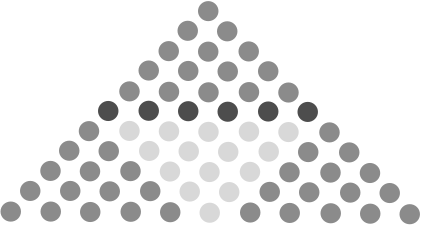
\includegraphics[scale=0.5]{FiguresMaths/Delta4}
 \caption{Arranging the four triangles plus a row to obtain a new (bigger) triangle.}
       \label{fig:Delta(n)4}
\end{center}
\end{figure}
Now, ``complete the picture'' by adding an ``extra'' row of $n$
tokens at row $n$ of the figure (these are depicted in dark gray in
the figure).  The four small triangles, augmented by the ``extra'' row
of $n$ tokens has clearly become a representation  of $\Delta_{2n-1}$
by tokens.

We now have a purely pictorial proof of the proposition. 
\medskip

\noindent \textit{Lesson learned.}

Training.


\subsection{A variant for computing the sum of the first integers $\Delta_n$}

\noindent \textit{The aim.}

Application of geometric sum.
\medskip

\noindent \textit{The problem.}

%Compute the sum of the first integers $\Delta_n$. 
Show graphically that $\Delta_n$ (sum of the first $n$ integers) is congruent to $1$ modulo $8$.
\medskip

\noindent \textit{Hint.}
Write the previous relation as $8 \Delta_n = K^2 -1$
for an integer $K$ to determine and represent the square $K$ by $K$. 

\noindent \textit{The solution.}

The expression $8 \Delta_n = (2n-1)^2 -1$ can be represented as in~\ref{fig:Sum8deltas}.
\begin{figure}[ht]
\begin{center}
       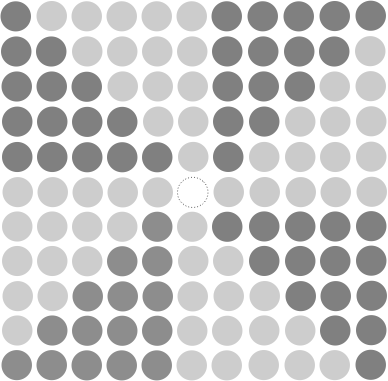
\includegraphics[scale=0.4]{FiguresMaths/Delta8}
\caption{8 copies of $\Delta_n$ are filling a big square but one token.}
       \label{fig:Sum8deltas}
\end{center}
\end{figure}


\subsection{On meeting new people}

\noindent \textit{The aim.}
Illustration of pigeon's hole principle.
\medskip

\noindent \textit{The problem.}
You are attending a cocktail party that is populated by $n$ couples.
In order to create a warm atmosphere, the host requests that each
attendee shake the hand of every attendee that he or she does not
know. \\
Prove that some two attendees shake the same number of hands.
\medskip

\noindent \textit{The solution.}
%
This observation follows from the \textit{pigeonhole principle}:
If $n+1$ pigeons occupy $n$ pigeonholes, then some hole contains
at least $2$ pigeons.
{\Denis is it useful to recall the principle here? I don't think so...}

This principle guarantees that some two attendees shake the same
number of hands.  To wit, the number of people that each attendee {\em
  does not know} belongs to the set $\{ 0, 1, \ldots, 2n-2 \}$,
because each person knows him/herself and his/her partner.  Because
there are $2n$ handshakers (the pigeons) and $2n-1$ numbers of hands
to shake (the boxes), some two shakers must shake the same numbers of
hands. 
\medskip

\noindent \textit{Lesson learned.}
Training for mastering different types of proofs, here the focus is put on Pigeonhole.


%%%%%%%%%%%%%%%%%%%%%%%%%%%%%%%%%%%%%%%

\subsection{A graphical proof for a specific geometric series}

\noindent \textit{The aim.}
To develop more intuition in solving using geometrical arguments.

Particular case of geometric series.
\medskip

\noindent \textit{The problem.}
Compute the sum of $(\frac{1}{4})^k$ using a graphical argument ($k \geq 0$).
\medskip

\noindent \textit{The solution.}
A rapid analysis of the small values of $k$ leads to the guess $(\frac{1}{4})^k = \frac{1}{3}$.
 
The solution is depicted in Fig.~\ref{Fig:Sumgeo1sur4}. 
\begin{figure}
\begin{center}
        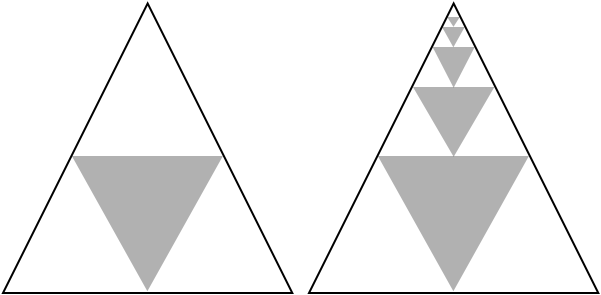
\includegraphics[scale=0.3]{FiguresArithmetic/SumGeometric1sur4}
        \caption{Graphical construction. Assuming the total area is 1, the area of the grey internal triangle (left) is $\frac{1}{4}$.
        As the grey area is one third at each layer (right), the whole area is $\frac{1}{3}$.
        By the double counting Fubini's principle, this area is the sum of the $\frac{1}{4^k}$ (for $k \geq 1$).}
        \label{Fig:Sumgeo1sur4}
\end{center}
\end{figure}

Finding such a triangular pattern may not be considered as an easy task.
However, as stated in the problem, the main point is to divide an elementary surface
into four equal pieces. 
Squares (or even worse disks) are not simple to use in this context while isosceles triangles 
are a \textit{natural} structure. 
\medskip

\noindent \textit{Lesson learned.}
Training and gain intuition for mastering geometrical proofs. 


%%%%%%%%%%%%%%%%%%%%%%%%%%%%%%%%%%%%%%%%%%%%%%


\section{Chapter 3. Sets}

%%%
\subsection{Operation on sets}

\noindent \textit{The problem.}

Define the following two operations from union and set
difference: {\it intersection} ($S \cap T$), which isolates all
elements shared by sets $S$ and $T$, and {\it symmetric difference}
($S+T$), which isolates all elements that belong to precisely one of
$S$ and $T$.
\medskip

\noindent \textit{The solution.}
{\Denis Do we have to answer this exercice?}


%%%
\subsection{Link of equality and equivalence relation}

\noindent \textit{The problem:}
Provide a proof of Theorem~\ref{thm:equality=finest-equiv}:

The equality relation, $=$, on a set $S$ is the {\em finest}
equivalence relation on $S$, in the sense that $=$ refines every
equivalence relation on $S$.
\medskip

\noindent \textit{The solution.}
Apply the definitions. 


%%%
\subsection{Propositional logic}

\noindent \textit{The problem.}
After consulting Fig.~\ref{fig:defns-via-tables}:

\begin{tabular}{llcl}
1. &
{\it Prove that the Propositional expression} &
$\sim P \ \Rightarrow \ P$ &
{\it is a tautology.} \\
2. &
{\it Prove that the Propositional expression} &
$P \ \Rightarrow \ \sim P$ &
{\it is satisfiable.}
\end{tabular}

%%%
\subsection{More on SAT}

\noindent \textit{The problem.}

Prove that the views of SAT are equivalent: (1) a set of clauses; (2)
a disjunction of clauses.



%%%
\section{Chapter 4. Numbers I}

\subsection{Complex
  multiplication via $3$ real multiplications}
\index{complex number!multiplication via 3 real multiplications}

\noindent {\it The problem.}
%\label{thm:complex-mult-3real}
Show how to compute the product of two complex numbers using only {\em three}
real multiplications rather than four.
\medskip

\noindent {\it The solution.}
Although implementing (\ref{eq:complex-mult}) ``directly'' correctly
produces the product $\kappa = (a+bi) \cdot (c+di)$, there is another
implementation that is {\em more efficient}.  Specifically, the
following recipe computes $\kappa$ using only {\em three} real
multiplications instead of the four real multiplications of the
``direct'' implementation.  We begin to search for this recipe by
noting that our immediate goal is to compute both Re$(\kappa) = ac-bd$
and Im$(\kappa) = ad+bc$.  We can accomplish this by computing the
{\em three} real products
\begin{equation}
\label{eq:complex-mult-3a}
(a+b) \cdot (c+d); \ \ \ \ \
ac;  \ \ \ \ \ bd
\end{equation}
and then noting that
\begin{equation}
\label{eq:complex-mult-3b}
\begin{array}{lcl}
\mbox{Im}(\kappa) & = & (a+b) \cdot (c+d) - ac -bd, \\
\mbox{Re}(\kappa) & = & ac -bd
\end{array}
\end{equation}
We thereby achieve the result of the complex multiplication described
in (\ref{eq:complex-mult}) while using only {\em three} real
multiplications.


%%%
\subsection{Another proof for irrationality of $\sqrt{2}$}


\noindent \textit{The problem.}
Prove the irrationality of $\sqrt{2}$ using a geometrical argument.
\medskip

\noindent \textit{Hint.}
The proof is by contradiction. 

Consider $\sqrt{2}$ is rational, which means there exists a pair of integers $(a,b)$
such that $\sqrt{2} = \frac{a}{b}$ (where $a$ is larger than $b$).
Among all possible pairs, take the unique irreductible ratio.

Represent this expression geometrically by the corresponding isosceles triangle
which is the one of minimal surface. 

The contradiction comes by constructing another isosceles triangle with a smaller surface.
%Squaring this expression leads to $2.b^2 = a^2$.
\medskip

\noindent \textit{The solution.}

The solution is depicted in Fig.~\ref{Fig:sqrtbisInit} and~\ref{Fig:sqrtbisFin} . 
\begin{figure}
\begin{center}
        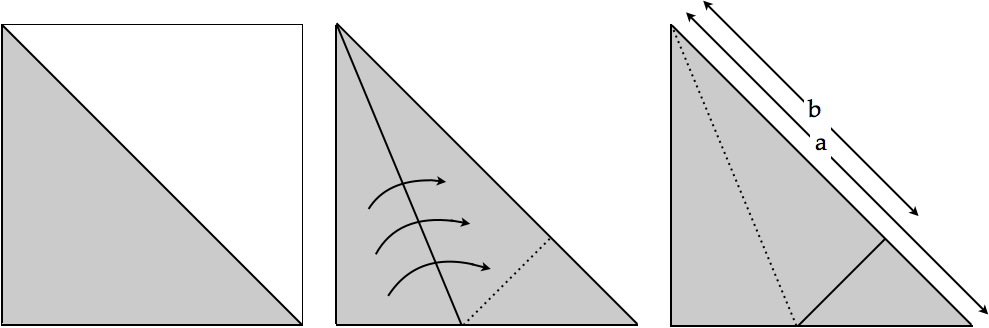
\includegraphics[scale=0.3]{FiguresArithmetic/sqrtbisInit}
        \caption{First step: folding the triangle along the side.}
        \label{Fig:sqrtbisInit}
\end{center}
\end{figure}
\begin{figure}
\begin{center}
        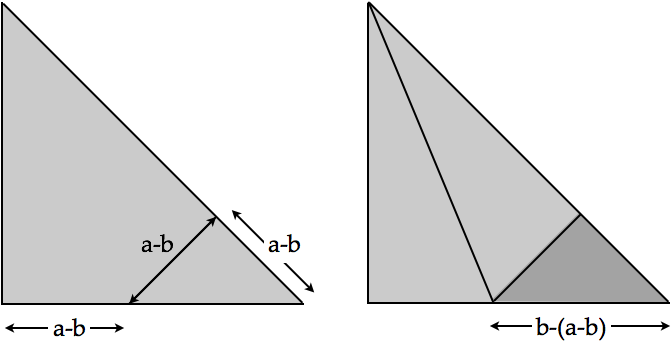
\includegraphics[scale=0.3]{FiguresArithmetic/sqrtbisFin}
        \caption{Second step. The sides of the small isosceles triangle are integers.}
        \label{Fig:sqrtbisFin}
\end{center}
\end{figure}



%%%%%%%%%%%%%%%%%%%%%%%%%%%%%%%%

\section{Chapter 5. Arithmetic}


\subsection{A ``trick'' for squaring certain integers}


\noindent \textit{The problem:}

Let $n$ be any number that has a $2$-digit decimal numeral of the form

\hspace{.25in}$5.\delta$ \ \ \ \ $(\delta \in \{ 0,1,2,3,4,5,6,7,8,9\})$.

\noindent
Then the square of $n$ is the integer

\hspace{.25in}$25 \ + \ \delta \cdot (\delta +1)$
\medskip

\noindent \textit{The solution:}

We can rewrite the premise of the proposition in the form
\[ n \ = \ 10 \cdot \delta + 5 \]
It is now easy to invoke Proposition~\ref{prop:(a+b)(c+d)} and the
distributive law to compute that

\[ n^2 \ = \ 100 \cdot \delta \cdot (\delta+1) + 25 \]
To wit: 
\[
\begin{array}{lclll}
n^2 & = & (10 \cdot \delta + 5)^2 & & \mbox{Given} \\
    & = & 100 \cdot \delta^2 \ + \ 100 \cdot \delta \ + \ 25
              & & \mbox{the proposition} \\
    & = & 100 \cdot (\delta^2 \ + \ \delta) \ + \ 25
              & & \mbox{factoring: distributive law} \\
    & = & 100 \cdot \delta \cdot (\delta + 1) \ + \ 25
              & & \mbox{factoring: distributive law} \\
\end{array}
\]
A parlor trick has become a mathematical demonstration!


%%%
\subsection{Revisiting a very old problem}

\noindent \textit{The problem:}

This problem comes from babylonians in the 18th century BC.
The numeral system was in base 60, and the problem was to determine the length of the side of a square which was part of a larger rectangle.
The following figure details the process.
\medskip

\noindent \textit{The solution:}

The idea of the proof is to represent the left hand side by the square $x^2$ beside a rectangle $60 \times x$
(see Fig.~\ref{fig:equationBabillon}).
Recall that the coefficient of $x$ in the equation is $1$, this corresponds to $60$ in the considered basis. 
Then, split the right rectangle into two equal parts and move one part a the bottom of the left square.
The final figure shows the whole square whose surface is equal to $45$ plus the surface of the white square
whose surface is equal to $30 \times 30$.
In base $60$, this is equal to $15$. 
$45+15 = 60$, thus, the big square is the unit square, its side is $60$.
Thus, the length of the initial square is equal to $60-30=30$.
\begin{figure}[htb]
\begin{center}
       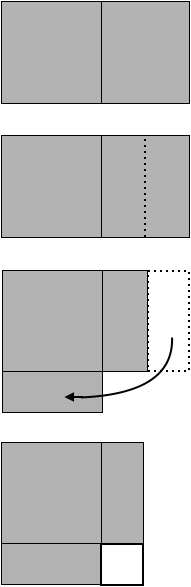
\includegraphics[scale=0.4]{FiguresArithmetic/tabletteMesopotamie}
\caption{Solving $x^2 + x = 45$.}
\label{fig:equationBabillon}
\end{center}
\end{figure}


%%%%%%%%%%%%%%%%%%%%%%%%%%%%%%%%%%%%%%%%%%

\section{Chapter 6. Summations}


\subsection{Compute $\Delta_n$ by means of sum of squares}

\noindent \textit{The problem.}
$\Delta_n = \sum_{i=1}^{n} i = \frac{n(n+1)}{2}$
\medskip

\noindent \textit{The solution.}

The idea here is to write the sum by extracting the first and the last element
of the sum of squares.
%We loose since the coefficient of the $\Delta_n$ is the same after these manipulations, but we can manage if we compute the \textit{next} sum, that is sum of the squares.
\medskip

$S_{n+1} = 1 + \sum_{i=1}^{n+1} i^2$

$S_{n+1} = (\sum_{i=1}^{n} i^2) + (n+1)^2$

where $\sum_{i=1}^{n+1} i^2 
= \sum_{i=0}^{n} (i-1)^2 
= \sum_{i=0}^{n} (i^2-2i+1) 
= \sum_{i=0}^{n} i^2- 2 ( \sum_{i=0}^{n} i) + (n+1)
= \sum_{i=1}^{n} i^2- 2 ( \sum_{i=1}^{n} i) + (n+1)$

Thus, 
$\sum_{i=1}^{n} i^2- 2 ( \sum_{i=1}^{n} i) + (n+1) = (\sum_{i=1}^{n} i^2) + (n+1)^2$

$-2 \Delta_n + (n+1) =  (n+1)^2$

$\Delta_n =  (n+1)^2-(n+1) = n(n+1)$

%%%
\subsection{Training on undetermined coefficient method}

\noindent \textit{The problem.}
Say that you are told that the sum of the first $n$ perfect squares is
a {\em cubic} polynomial in $n$.  Use the method of undetermined
coefficients to derive the exact formula (\ref{eq:sum-1-to-nsq1}) for
the sum.
\medskip

\noindent \textit{The solution.}

to be done


%%%
\subsection{Tetrahedral numbers}


\noindent \textit{The problem.}
Prove the following expression

$\Theta_n =  \sum_{k=1}^{n} \Delta_k = \frac{n.(n+1).(n+2)}{6}$
\medskip

\noindent \textit{Hint.}
This result can easily been proved by recurrence, we let the reader develop it. 
We suggest to use the double counting Fubini's principle.

Following this way, you should write the previous expression of the tetrahedral number in a developed form 
using a triangle shape as shown in Fig.~\ref{fig:TetrahedralBasic}.
\begin{figure}[h]
\begin{center}
        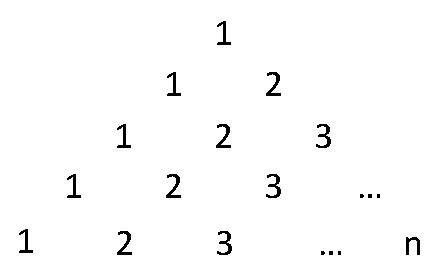
\includegraphics[scale=0.5]{FiguresArithmetic/TetrahedralBasic}
        \caption{Computing $\Theta_n$: basic triangle pattern.}
        \label{fig:TetrahedralBasic}
\end{center}
\end{figure}
and draw two copies by rotating the dimensions.

Fubini's principle is used by summing up the successive rows.

Prove as an intermediate result that the sum of the elements over the rows of the three triangles is proportional to $n+2$.
\medskip

\noindent \textit{The detailed solution.}
We proved the expression of $\Delta_n$ by mirroring the developed expression and adding term by term.
Similarly, a way to prove the expression of $\Theta_n$ is to consider three copies and organize them 
in order to obtain the expected result.
A tetrahedral number can be arranged as a triangle (see Fig.~\ref{fig:TetrahedralBasic}).
%\begin{figure}[h]
%\begin{center}
%        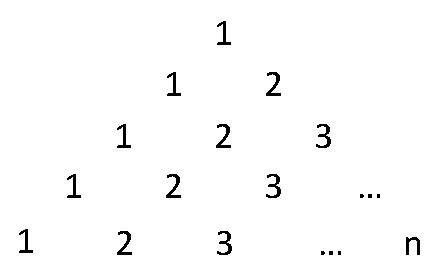
\includegraphics[scale=0.5]{FiguresArithmetic/TetrahedralBasic}
%        \caption{Computing $\Theta_n$: basic triangle pattern.}
%        \label{fig:TetrahedralBasic}
%\end{center}
%\end{figure}

The proof is obtained by the double counting principle by rotating the three faces of triangles as shown in Fig.~\ref{fig:Tetrahedral}.
\begin{figure}[h]
\begin{center}
        \includegraphics[scale=0.5]{FiguresArithmetic/Tetrahedral}
        \caption{Computing $\Theta_n$ using an adequate arrangement of $3$ triangles.}
        \label{fig:Tetrahedral}
\end{center}
\end{figure}

Sum up all the numbers in each row.

\begin{itemize}
\item 
The first row is equal to $1+1+n = n+2$.
\item
The second one is equal to $3 + 3 + 2(n-1) = 2(n+2)$. 
\item
Let us sum up the elements in row $k$: 

$\Delta_k + \Delta_k + k(n-k+1)  = k(k+1) + kn-k^2+k = k(n+2)$.
\end{itemize}

Conclusion:
the global sum is equal to $n+2$ times $(1+2+...+n)$.

Finally, $3 \Theta_n = (n+2) \Delta_n$.
\medskip

\noindent \textit{Going further.}

Summary: we proved the following results:
\begin{itemize}
\item $Id_n = 1+1+ ... +1 = n$
\item $\Delta_n = 1+2+3+ ... +n = \frac{1}{2}.Id_n.(n+1)$
\item $\Theta_n = \Delta_1 + \Delta_2 + ... + \Delta_n = \frac{1}{3} .\Delta_n.(n+2)$
\end{itemize}

A natural question is if we can go further following the same pattern for computing 
$ \sum_{k=1}^{n} \Theta_k$, and so on.

Are you able to consider the challenge?


%%%
\subsection{Sum of perfect cubes}

\noindent \textit{The problem.}
Show that the sum of $n$ first cubes is equal to a perfect square, and more precisely, $\Delta_n^2$.
\medskip

\noindent \textit{The solution.}
The proof is based on an hold and simple pattern that we learned in elementary school.
\medskip

\index{$n^2$ as sum of first $n$ odd integers!a proof from elementary school}

%
Consider the following reasoning which emerges from the way
multiplication tables are developed in elementary school.  
Let us first illustrate the idea using the case $n=5$.
\begin{equation}
\label{eq:Fubini-table}
\begin{array}{rrrrr}
1  &  2 &  3 &  4 &  5 \\
2  &  4 &  6 &  8 & 10 \\
3  &  6 &  9 & 12 & 15 \\
4  &  8 & 12 & 16 & 20 \\
5  & 10 & 15 & 20 & 25 \\
\end{array}
\end{equation}
Write the integers $1, 2, \ldots, n$ in a row.  Below this row, write
the doubles of these integers.  Below the ``double'' row, write the
triples of the integers.  Below the ``triple'' row, write the
quadruples of the integers, then the quintuples, and so on.  Note that
the resulting table is {\em symmetric:} its rows are identical to its
columns.
\medskip

Using again Fubini's rearrangement stratagem, we now count all the integers in
the table in two different ways.
\begin{enumerate}
\item
We sum the entries of our table by peeling away successively larger
reversed instances of the letter ``$L$'' (as in our earlier
``pictorial'' proof of
Proposition~\ref{thm:squares-odd-integers-Gauss}).  We find that the
integers in each ``$L$'' sum to a perfect cube.
Actually, the diagonal is (by definition) equals to the square.
\[
\begin{array}{rrrrrrrrr|rrc}
1  &    &    &    &    &   &     &    &   & 1   & = 1^3 \\
2  &  4 &  2 &    &    &   &     &    &   & 8   & = 2^3 \\
3  &  6 &  9 &  6 &  3 &   &     &    &   & 27  & = 3^3 \\
4  &  8 & 12 & 16 & 12 &  8 &  4 &    &   & 64  & = 4^3 \\
5  & 10 & 15 & 20 & 25 & 20 & 15 & 10 & 5 & 125 & = 5^3
\end{array}
\]

\item
We sum the successive rows of the $n \times n$ table (\ref{eq:Fubini-table}).  
The first row of the table sums to $\Delta_n$; the second row sums to $2
\Delta_n$; the third row sums to $3 \Delta_n$; \ldots; the last row sums
to $n \Delta_n$.  
Thus, the aggregate sum of the table's rows is 
\[ (1 + 2 + \cdots + n) \cdot \Delta_n \ = \ \left(\Delta_n \right)^2 \]
\end{enumerate}
We conclude that
\[
\sum_{i=1}^n i^3 \ = \  \left(\Delta_n \right)^2
\]



\subsection{Harmonic series}

\noindent \textit{The problem}

Show that the harmonic series $H_n =  \sum_{k=1}^{n} \frac{1}{k}$ diverges (it goes to infinity).
\medskip

\noindent \textit{The solution.}
The analysis is as follows.

A first solution is to group the terms according to powers of $2$. 
Then, the sum within each group is between $\frac{1}{2}$ and $1$, thus,
$H_n > \frac{1}{2}.n$
\medskip

Another (more precise) way is to gather the terms 3 by 3 as follows:

$S_k = (\frac{1}{3k-1} + \frac{1}{3k} + \frac{1}{3k+1} )$ for $k\geq1$, 

$H = 1 + S_1 + ... + S_k + ... > 1 + 3.\frac{1}{3} + 3.\frac{1}{6} + ... + 3.\frac{1}{3k} + ... $

since $S_k > 3.\frac{1}{k} $.

The proof is by contradiction:

if $H$ is finite, from the previous relation we have: $H > 1 + H$, which is obviously impossible.
\medskip

Moreover, the first way of  bounding the sum tells us about its value (actually, we know the value at a factor of $2$):

$\frac{log(n)+1}{2} < H_n < log(n)+1$. Thus, $H_n = O(log(n))$



%%%%%%%%%%%%%%%%%%%%%%%%%%%%%%%%%%%%%

\section{Chapter 7. Infinity}

\subsection{Handling asymptotic}


\noindent \textit{The problem.}

Prove that $f = O(g)$ and $h = O(k)$ for functions $f,g,h,k$ implies that
$f+h = O(g+k)$
\medskip

{\Denis no need to write a solution}


\subsection{What's wrong?}

\noindent \textit{The aim.}
to investigate a proof which leads to surprising results.


\begin{enumerate}
\item
Let consider the infinite sum $A = 1-1+1-1+ \ldots$

show that $A=\frac{1}{2}$ (hint: compute $1-A$)
\item
Let now consider the other infinite sum $B=2-3+4-5+6 \ldots$

show that $B=\frac{1}{4}$ (hint: compute $A+B-1$)
\item 
Compute the sum of the integers $C=1+2+3+4+ \ldots$

show that $C=-\frac{1}{12}$ (hint: compute $C-B=4+8+12+16+ \ldots$)
\end{enumerate}

\medskip

\noindent \textit{The problem.}

What's wrong?

\medskip

\noindent \textit{The solution.}
First, summing up positive number should be positive, 
and second, the sum of the integers should be infinite...

Then, how to analyze the previous result/proof?
{\Denis classical result, detail its analysis}





%%%%%%%%%%%%%%%%%%%%%%%%%%%%%%%%%%


\section{Chapter 8. Numbers II divisibility}

\subsection{A simple exercice on divisibility}

\noindent \textit{The problem:}

Every integer $n>1$ is divisible by at least one prime number.

{\Denis no solution needed here, I am still skeptical about its relevance...}


\subsection{Numerals and divisibility}

\noindent \textit{The problem:}
Prove that when you do Euclidian division, then the {\em remainder}
upon each consecutive division is the next lowest-order digit in the
base-$b$ numeral for $n$.
\medskip

\noindent \textit{The solution:}

Do we have to give the solution?


\subsection{A fun result dealing with divisibility}

\noindent \textit{The problem:}
Let consider the $2n$ first integers.

Take any $n+1$ integers in this set and prove that there exists a pair $(p,q)$
such that $p$ divides $q$. 
\medskip


\noindent \textit{The solution:}

%This exercice was a favorite question by the famous mathematician Paul Erdos,
%he often used it to test the ability of young students in mathematics...
%\medskip

%Use the pigeon hole principle to exhibit $p$ and $q$.


Let $\alpha_i$ be the elements of this set of $n+1$ elements.
Write $\alpha_i = 2^k \times m$ where $m$ is odd (and $k \geq 0$).

The $2n$ numbers of the sequence are decomposed into multiples of powers of $2$.
When there are multiple ways, we take the one with the largest power of $2$ in order to make the decomposition unique.
Example for $n=7$:

1, 3, 5, 7, 9, 11, 13

2, 6, 10, 14

4, 12

8
\medskip


%The sketch of the proof is as follows.
\begin{enumerate}
\item
 $\alpha_i = 2^k \times m$ 
 
$m$ belongs to the $n$ numbers $\{1,3,5, \ldots, 2n-1 \}$

As we are considering $n+1$ integers, from the pigeon hole principle, there are two numbers with the same value of $m$. 
\item 
Thus, $2^{k1} \times m$ and $2^{k2} \times m$

$p$ is the smallest one, which divides $q$ (the largest one).
\end{enumerate}


\subsection{When is integer $n$ divisible by $9$?}
\label{sec:divisible-by-9}

%\noindent \textit{The aim.}
%
%We exploit here our ability to evaluate geometric summations to
%illustrate a somewhat surprising, nontrivial fact.  One can deduce
%information about the divisibility of an integer $n$ from $n$'s
%positional numerals.  We hope that this ``fun'' result will inspire
%the reader to seek kindred numeral-encoded properties of numbers.
%
%\medskip
\noindent \textit{The problem.}
%\label{thm:div-by-b-bar}
An integer $n$ is divisible by an integer $m$ if, and only if, $m$
divides the sum of the digits in the base-$(m+1)$ numeral for $n$.
%\medskip
%
%The most familiar instance of this result is phrased in terms of our
%traditional use of base-$10$ (decimal) numerals. \\
%{\it An integer $n$ is divisible by $9$ if, and only if, the sum of
%  the digits of $n$'s base-$10$ numeral is divisible by $9$.}
\medskip

\noindent \textit{The solution.}

({\it Argument for general number-base $b$}).
%
Of course, we lose no generality by focusing on numerals without
leading $0$'s, because leading $0$'s do not alter a numeral's sum of
digits.

Let us focus on the base-$b$ numeral for a number $n$ (so $b = m+1$ in
the statement of the proposition).  There therefore exist base-$b$
digits---i.e., integers from the set $\{0, 1, \ldots, b-1\}$---call
them $\delta_k \neq 0$, $\delta_{k-1}$, \ldots $\delta_1$, $\delta_0$,
such that
\[ n \ = \ \delta_k \cdot b^k + \delta_{k-1} \cdot b_{k-1} + \cdots +
\delta_1 \cdot b + \delta_0. \]
The sum of the digits of $n$'s base-$b$ numeral is, then
\[ s_b(n) \ \eqdef \ \delta_k + \delta_{k-1} + \cdots + \delta_1 +
\delta_0. \]
Let us calculate the difference $n - s_b(n)$ in the following manner,
digit by digit.
\begin{equation}
\label{eq:sum-of-digits}
\begin{array}{ccccccccccc}
n & = &
\delta_k \cdot b^k & + & \delta_{k-1} \cdot b^{k-1} & + & \cdots
  & + & \delta_1 \cdot b & + & \delta_0 \\
s_b(n) & = &
\delta_k & + & \delta_{k-1} & + & \cdots & + & \delta_1 & + & \delta_0 \\
\hline
n - s_b(n) & = &
\delta_k \cdot (b^k -1) & + &
\delta_{k-1} \cdot (b^{k-1} -1) & + &
\cdots & + &
\delta_1 \cdot (b-1) & & 
\end{array}
\end{equation}

We now revisit summation (\ref{eq:geom-sum:b>1}).  Because $b$ is a
positive integer, so that $1 + b + \cdots + b^{a-2} + b^{a-1}$ is also
a positive integer, we infer that {\em the integer $b^a -1$ is
  divisible by $b-1$.}

We are almost home.  

Look at the equation for $n - s_b(n)$ in the
system (\ref{eq:sum-of-digits}).  As we have just seen, every term on
the righthand side of that equation is divisible by $b-1$.  It follows
therefore, that the lefthand expression, $n - s_b(n)$, is also
divisible by $b-1$.
An easy calculation, which we leave to the reader, now shows that this
final fact means that $n$ is divisible by $b-1$ if, and only if, $s_b(n)$ is.


\subsection{Modulus arithmetic}

\noindent \textit{The problem:}
$\N_q$ is never closed under the operation of division when the modulus $q$ is composite.
\medskip

\noindent \textit{The solution:}


%%%%%%%%%%%%%%%%%%%%%%%%%%%%%%%%%%%%%%%%%


\section{Chapter 9. Recurrences}

\subsection{Karatsuba Multiplication} 

\noindent \textit{The aim.}
The purpose here is to put the Master theorem (section~\ref{sec:linear-recurrence-general}) in action on a classical problem.

\medskip

The classical elementary-school method for computing the base-$2$ product of two $n$-bit integers (using their standard numerals)
\[ A \ = \ a_{n-1} a_{n-2} \cdots a_0 \ \ \ \ \mbox{ and } \ \ \ \ B \ = \ b_{n-1} b_{n-2} \cdots b_0 \]
is to compute the $n$ partial products:
\[ (a_{n-1} a_{n-2} \cdots a_0) \times b_i 2^i \]
and to sumthese partial products.

This approach leads to $O(n^2)$ basic operations. 

\medskip

We can do better.

\medskip

Let us first recall the generic divide-and-conquer for designing algorithms.
\bigskip

\noindent \fbox{
\begin{minipage}{0.95\textwidth}
{\it Divide and conquer} is a paradigm for designing efficient algorithms for solving problems that can be decomposed into sub-problems.

Let consider a problem of size $n$ that can be decomposed into $p$ sub-problems.
(notice, all sub-problems have the same size $n/q$).

\bigskip

\noindent {\bf Principle:}
\begin{enumerate}
\item Decompose the problem into $a$ sub-problems of size $\frac{n}{q}$.
\item Solve those sub-problems.
\item Reconstruct the solution of the initial problem.
\end{enumerate}

In general, the sub-problems are solved recursively (at least until a certain threshold value of the parameter, where the base case(s) govern the computation).

The time-cost of the computation is governed by the following expression:
\[  T(n) \ = \ p \cdot T(\frac{n}{q}) + c_1(n) + c_3(n) \] 
where $c_1(n)$ and $c_3(n)$ are the costs of phases (1) and (3).
\end{minipage}
}
\bigskip

\noindent \textit{The problem.}
Say that we have the earlier-mentioned $n$-bit numbers $A$ and $B$.  Let us assume that $n$ is a very large power of $2$: $n=2^k$ for some positive integer $k$.

The goal is to compute the product $A \times B$ in fewer operations than the classic $O(n^2)$.

\medskip

\noindent \textit{A first solution.}
The divide-and-conquer version of this problem is to break each integer into two parts
of $n/2$ bits each:

$A=(a_n\ldots a_{n/2+1})_2 2^{n/2}\ + (a_{n/2}\ldots a_1)_2$

Denoting by $A_1$ and $A_2$ the two separate terms, we get:

$A.B = (A_1.B_1) 2^n + (A_1.B_2 + A_2.B_1) 2^{n/2} + A_2.B_2$
\medskip

The previous computation requires 4 multiplications of integers of $n/2$ bits 
and 3 additions of integers with at most $2n$ bits. The multiplication of integers in base 2 by powers of 2 
correspond to simple shifts to the left. 

The cost is given by the following expression: $T(n) = 4.T(\frac{n}{2}) + f(n)$ where $f$ is a linear function
and $T(1) = 1$.

We obtain $T(n) = \Theta(n^2)$, same as for the naive algorithm.
\bigskip
 
\noindent \textit{The second problem:}
The idea of Karatsuba is to decrease the number of multiplications 
(at the price of slightly increasing the additions/subtractions) by using the following identity:

$A_1.B_1 + A_2.B_2 + (A_1-A_2).(B_2-B_1)$

Show how to use this relation and develop the cost analysis of this algorithm.
\medskip

\noindent \textit{The solution.}

The relation is easy to check and it is left to the reader. 
Let us use it and replace in the original expression:

$A.B = (A_1.B_1) 2^n + (A_1.B_1 + A_2.B_2 + (A_1-A_2).(B_2-B_1)) 2^{n/2} + A_2.B_2$

The cost analysis is 3 multiplications of $n/2$ bits,
4 additions and 2 subtractions of integers at most $2n$ bits. 

Again, using the Master Theorem leads to:

$T(n) = 3.T(n/2) + \Theta (n) = n^{\log_2 3}$



\subsection{Computing Fibonacci Numbers Fast}
\label{sec:FastFibo}

\noindent \textit{The aim.} 
Show a new computational scheme for the Fibonacci numbers.

Notice that it is generic and related to the scheme of fast exponentiation.
\medskip


\noindent \textit{The problem.} Verify the following expression and develop an argument for its interest.

$F(2n) = F(n)^2 + F(n-1)^2$

$F(2n+1) = (2.F(n-1) + F(n)).F(n)$
\medskip

\noindent \textit{The solution.}

The proof is by induction.

The basis case is obtained for $n=1$.
It is true since:

$F(2) = F(1)^2+F(0)^2 = 2$

$F(3) = (2.F(0)+F(1)).(F(1)) = 3$
\medskip

Let assume for proving the induction step that the property holds at rank $n$ for both $F(2n)$ and $F(2n+1)$ and compute $F(2(n+1))$:

Apply first the definition of Fibonacci numbers: 

$F(2n+2) = F(2n+1)+F(2n)$ 

Replace both terms by the recurrence hypothesis:

$= F(n)^2 + F(n-1)^2 + (2.F(n-1) + F(n)).F(n)$

$= F(n)^2 + F(n-1)^2 + 2.(F(n).F(n-1)) + F(n)^2$

$= (F(n) + F(n-1))^2 + F(n)^2$

We obtain the result by applying again the definition of Fibonacci numbers at order $n+1$:

$F(2(n+1)) = F(n+1)^2 + F(n)^2$
\medskip

The second part of the proposition is obtained by applying the definition of Fibonacci numbers:

$F(2(n+1)+1) = F(2(n+1)) + F(2n+1)$

and replace both terms by their expressions respectively :

$= F(n+1)^2 + F(n)^2 + (2.F(n-1) + F(n)).F(n)$

$= F(n+1)^2 + 2.(F(n-1) + F(n)).F(n)$

$= F(n+1)^2 + 2.F(n+1).F(n)$
\medskip

We provide in Fig.~\ref{fig:fastFibo} a pictorial argument to show why this decomposition 
is particularly fast while computing Fibonacci numbers:
each $F(n)$ is computed in $log_2 (n)$ steps.
\begin{figure}[h]
\begin{center}
        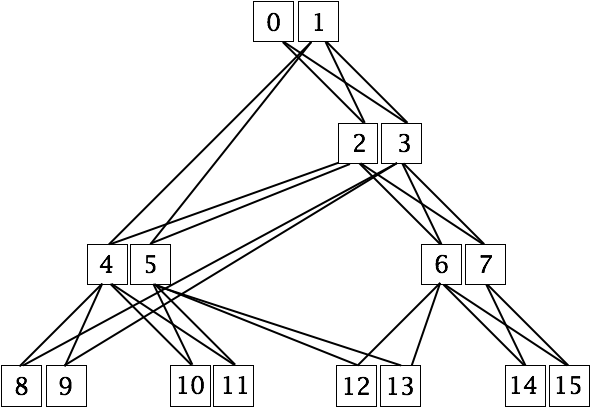
\includegraphics[scale=0.4]{FiguresMaths/FiboFast.png}
        \caption{Dependency relations for computing the pairs $(F(2n),F(2n+1))$.}
                \label{fig:fastFibo}
\end{center}
\end{figure}
In particular, we show how to compute an element ($F(13)$) using the fast Fibonacci scheme in Fig.~\ref{fig:fastFibo13}.
The pattern is embedded into a complete binary tree of predecessors (with some redundancies)
whose depth is logarithmic.
\begin{figure}[h]
\begin{center}
        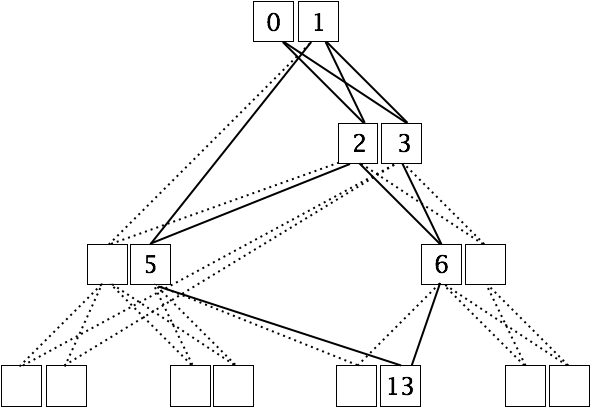
\includegraphics[scale=0.4]{FiguresMaths/FiboFast13.png}
        \caption{Ancestors involved in the computation of $F(13)$. }
        \label{fig:fastFibo13}
\end{center}
\end{figure}

The conclusion is that
any Fibonacci number $F(n)$ can be computed very fast in $log_2 (n)$ steps.



\subsection{Cassini's Identity}

\noindent \textit{The aim.}
Prove a classical identity involving Fibonacci numbers, which is a nice example of proof by recurrence.
\medskip

\noindent \textit{The problem.}
Prove the following expression:

$F(n-1).F(n+1) = F(n)^2 + (-1)^{n+1}$ for $n \geq 1$
\medskip

%Let check the expression on the first ranks:
%
%$n=1$, $F(0).F(2) = F(1)^2 +1 = 2$
%
%$n=2$, $F(1).F(3) = F(2)^2 -1 = 3$
%
%$n=3$, $F(2).F(4) = F(3)^2 +1 = 10$
%
%$n=4$, $F(3).F(5) = F(4)^2 -1 = 24$
%
%...
%\medskip

\noindent \textit{The solution.}
The proof is by induction.

The basis case $n=1$ holds since $F(0).F(2) = F(1)^2 +1 = 2$.

The induction step is proved assuming the Cassini's identity holds at rank $n$.
Replace $F(n+2)$ by its definition in the expression:
 
$F(n).F(n+2) = F(n) (F(n+1)+F(n)) = F(n)^2 + F(n).F(n+1)$

Then, replace the last term using the recurrence hypothesis:

$F(n)^2 = F(n-1).F(n+1) - (-1)^{n+1} =F(n-1).F(n+1) + (-1)^{n+2} $

Thus,
$F(n).F(n+2) = F(n).F(n+1) + F(n-1).F(n+1) + (-1)^{n+2} = F(n+1) (F(n) + F(n-1)) + (-1)^{n+2}$ 

Apply again the definition of Fibonacci sequence $F(n) + F(n-1) = F(n+1)$, we obtain:

$F(n).F(n+2) = F(n+1)^2 + (-1)^{n+2}$

This concludes the proof. 


\subsection{Lucas Numbers} 

\noindent \textit{The aim.}
Fibonacci progression is the most popular and the most simple Definition of Lucas' numbers

\textbf{Definition.}
Given the two starting numbers $L(0) = 1$ and $L(1) = 3$, 
the other Lucas numbers are obtained by the same progression as Fibonacci: 

$L(n+1) = L(n)+L(n-1)$.
\medskip

In order to gain intuition on this problem, let us compute the first ranks in regard to the classical Fibonacci numbers:
\begin{figure}[htb]
\[
\begin{array}{c||r|r|r|r|r|r|r|r|r|r|r}
{\displaystyle n } & k=0 & k=1 & k=2 & k=3 & k=4 & k=5 &
k=6 & k=7 & k=8 & k=9 & \ldots \\
\hline
F(n) & 1 & 1 &  2  &  3  &   5  &   8  &  13  &  21  & 34  & 55  & \ldots \\
\hline
L(n) & 1 & 3 &  4 &  7  &  11  &  18  &  29 & 47  & 76  & 123 & \ldots \\
\hline
\end{array}
\] 
\caption{Correspondence between Fibonacci and Lucas numbers.}
\label{fig:fiboLucas}
\end{figure}
%
%n: $~~~~0, 1, 2, 3, ~4, ~5, ~6, ~7, ~8, ~~9, ...$
%
%F(n): $1, 1, 2, 3, ~5, ~8, 13, 21, 34, ~55, ...$
%
%L(n): $1, 3, 4, 7, 11, 18, 29, 47, 76, 123, ...$
\medskip

%
%There are strong links with Fibonacci numbers.
%In particular, we established before that
%\bigskip
%
%$F(n+2) = 1+ \sum_{k=0}^{n} F(k)$. 
%\bigskip
%
%We have similarly: $L(n+2) = 1+ \sum_{k=-1}^{n} L(k)$ since the basic step of the induction is still valid: 
%
%$L(2) = L(-1 )+L(0) +1 = 2+1+1 = 4$.
%%Actually, it will be true for all the progressions where $u_1=1$.
%

\noindent \textit{The problem.}
Prove the following expression:

$F(k-1).L(n) = F(n+k)+ (-1)^{k-1}F(n-k)$ for $k \leq n$
\bigskip

\noindent \textit{The solution.} 

There are two integers involved here ($k$ and $n$).
Let us study the expression step by step for successive values of $k$.
\medskip

\begin{itemize}
\item Starting smoothly with $k=1$

We can easily show by induction on $n$ that the Lucas number of order $n$ is the sum of two Fibonacci numbers:

$L(n) = F(n-1)+F(n+1)$ for $n \geq 1$
\medskip

%Let check this property on the first ranks:
%
%$n=2$, $L(2) = F(1)+F(3) = 1 + 3 = 4$
%
%$n=3$, $L(3) = F(2)+F(4) = 2 + 5 = 7$
%
%$n=4$, $L(4) = F(3)+F(5) = 3 + 8 = 11$
%
%$n=5$, $L(5) = F(4)+F(6) = 5 + 13 = 18$
%

The basis case, corresponding to for $n=1$) is true since $L(1) = 3 = F(2) + F(0) = 2+1$.

Let assume for proving the induction step that the property holds at all ranks $k \leq n$ and compute $L(n+1)$:

Apply the definition of Lucas' numbers: $L(n+1) = L(n)+L(n-1)$

Apply the induction hypothesis on both terms of the right hand side:

 $L(n+1) = F(n+1)+F(n-1)+F(n)+F(n-2)$

Apply now the definition of Fibonacci numbers for $F(n+1) + F(n) = F(n+2)$  and $F(n-1) + F(n-2) = F(n)$

Replace them in the previous expression:

$L(n+1) = F(n+2)+F(n)$

which concludes the proof.

\item
Extension.

Using a similar approach, we obtain $L(n) = F(n+2)-F(n-2)$. 
What happens if we generalize? Easy calculations lead to the following results:
\medskip

$2.L(n) = F(n+3) + F(n-3) $

%Proposition.
%
%$2.L(n) = F(n+3)+F(n-3)$
%\bigskip
%
%Proof.
%We start from $L(n) = F(n+2)-F(n-2)$
%
%$F(n+2) = F(n+3) - F(n+1)$ and $F(n-2) = F(n-1) - F(n-3)$
%
%$L(n) = F(n+3) - (F(n+1) + F(n-1)) + F(n-3)$
%
%$2.L(n) = F(n+3) + F(n-3)$
%
%
%\item Extension 2
%
%Go to the next step using the same technique:
%\medskip
%
%
%
%$= F(n+4) - F(n+2) + F(n-2) - F(n-4)$
%\medskip

$3.L(n) = F(n+4) - F(n-4)$

$5.L(n) = F(n+5) + F(n-5)$
\medskip
 
As $2, 3, 5$ are successive Fibonacci numbers, this gives us the intuition of the general case:

$F(k-1).L(n) = F(n+k) + (-1)^{k-1}F(n-k)$ for $k \leq n$
\medskip

which is proved (again) as follows by induction assuming the expression holds at rank up to $k$.

The basis case is straightforward (see case $k=1$).

Compute $F((k+1)-1).L(n)$ and apply the definition of Fibonacci number $F((k+1)-1) = F(k-1) + F(k-2)$

$F(k).L(n) = F(k-1).L(n + F(k-2).L(n)$ and replace both last terms by using the induction hypothesis:

$= F(n+k) + (-1)^{k-1}F(n-k) + F(n+k-1) + (-1)^{k-2}F(n-(k-1))$

$= F(n+k) +  F(n+k-1) + (-1)^{k-1}(F(n-k) - F(n-k+1))$

The final result is obtained by applying twice the definition of the Fibonacci numbers.
\medskip

\noindent \textit{Lesson learned.}
This exercice is a good example of the proof of a non straightforward recurrence which involves two integers.

\end{itemize}


\subsection{Binomial coefficients}

\noindent \textit{The aim:}

xx
\medskip

\noindent \textit{The problem:}

Prove Proposition~\ref{thm:pascal-binom} via the double induction
outlined in the text.



\subsection{La ruine}

\noindent \textit{The aim:}

Show a non natural bilinear recurrence.
\medskip

\noindent \textit{The problem:}

The goal here is to determine the values of  $U_n$

Solve $U_{n} = \frac{1}{2}.U_{n-1} + \frac{1}{2}.U_{n+1}$

knowing $U_0 = 0$ and $U_N = 1$
\medskip

\noindent \textit{The solution:}




\ignore{
*****\subsection{Lucas' numbers}

\noindent \textit{The problem.}

Prove the following expression.
 
$F(n+1) = \frac{1}{2} (F(0).L(n) + F(n).L(0))$
\medskip

\noindent \textit{The solution.}
The proof comes from direct arithmetic manipulations:

$2.F(n+1) = F(n+1) +  F(n+1) =  F(n+1) + F(n) + F(n-1)$

$= L(n) + F(n) $

$= F(0).L(n) + F(n).L(0)$
\medskip

\noindent \textit{The problem.}

The previous property can be extended for any $m>1$ as follows:
\medskip

$2.F(n+m) = F(m-1).L(n) + F(n).L(m-1)$
\medskip

\noindent \textit{The solution.}


The proof is by recurrence on $m$ considering any fixed $n$.
\begin{itemize}
\item
The \textbf{basis case} (for $m=1$) is given by the previous proposition.

\item
\textbf{Induction step:} 
Assume the property holds at rank $m > 1$ and consider $F(n+m+1)$:

Apply the definition of Fibonacci numbers: 

$F(n+m+1) = F(n+m)+F(n+m-1)$ 

Replace both terms by the recurrence hypothesis:

$= \frac{1}{2} (F(m-1).L(n) + F(n).L(m-1)) + \frac{1}{2} (F(m-2).L(n) + F(n).L(m-2))$

$= \frac{1}{2} \left( (F(m-1)+F(m-2)).L(n) + F(n).(L(m-1)+L(m-2))\right)$

$= \frac{1}{2} \left(F(m).L(n) + F(n).(L(m)\right)$
\end{itemize}
***** }

%%%%%%%%%%%%%%%%%%%%%%%%%%%%%%%%%%%%%%%%%

\section{Chapter 10. Numbers 3}

\subsection{Empty for the moment}

\subsection{Application of the Fundamental Theorem of Arithmetic}

\noindent \textit{The aim.}
Significant application of the Fundamental Theorem of Arithmetic~\ref{thm:Fund-Thm-Arith}.
\medskip

\noindent \textit{The problem.}
For all $\langle x,y \rangle \in \N^+ \times \N^+$

$\a(x,y) \ \eqdef \ 2^{x-1} \cdot (2y -1)$

verify function $\a$'s bijectiveness.
\medskip

\noindent \textit{The solution.}
xx
\medskip

\noindent \textit{Lesson learned.}



%%%%%%%%%%%%%%%%%%%%%%%%%%%%%%%%%%%%%%%%%

\section{Chapter 11. Combinatorics}

\subsection{Going further in a game analysis}

\noindent \textit{The problem:}
Analyze the game of craps in the same way as we did for sum-of-three

Verify the table in Fig.~\ref{fig:dice-ordered-configs}

In the ordered version of sum-of-three, sum$k$ is engendered by the
same number of configurations as is sum $21 - k$.  
Why is this the case?

\noindent \textit{The solution:}


\subsection{more about the Birthday paradox}

\noindent \textit{The aim:}
An interesting variant of the birthday puzzle
\medskip

\noindent \textit{The problem:}
Determine the
probability of a student to be born the same day as me.
\medskip

\noindent \textit{The solution:}



\subsection{A property about binomial coefficients}

\noindent \textit{The aim:}

xx
\medskip

\noindent \textit{The problem:}

Prove the following property by two ways (recurrence and by using a combinatorial argument

$\forall n,k$ $1 \leq k \leq n$

$k.{n \choose k} = n.{{n-1} \choose {k-1}}$
\medskip

\noindent \textit{The solution:}




%%%%%%%%%%%%%%%%%%%%%%%%%%%%%%%%%%%

\section{Chapters 12 and 13. Graphs}


{\Arny The proof of termination with a connected tree should be an
  exercise --- Phase 1 of the proof by deconstruction of Euler's
  formula} ---


\subsection{Formal definition of mesh graphs}
\label{Exercice:FormalDefinitionMesh}

\noindent \textit{The aim.}
The definition of mesh presented in chapter~\ref{ch:Graphs1}
is very easy to capture with a drawing.
We formalize here the precise definition using a mathematical language. 
\medskip

\noindent \textit{The problem.}
Formalize precisely the definition of mesh  $\m_{m,n}$ and torus $\widetilde{\m}_{m,n}$ graphs
for positive integers $m, n \in \N^+$.
\medskip

\noindent \textit{The solution.}
The  {\it vertex-set} is the same for both graphs:

\begin{eqnarray*}
\n_{\fm_{m,n}} \ = \ \n_{\widetilde{\fm}_{m,n}}
  & = & 
\{1, \ 2, \ldots, \ m\} \ \times \ \{1, \ 2, \ldots, \ n\} \\
  & = & 
\big\{ \langle i, \ j \rangle \ \ | \ \ 
\big[ i \in \{1, \ 2, \ldots, \ m\} \big], \ \
\big[ j \in \{1, \ 2, \ldots, \ n\} \big]
\big\}
\end{eqnarray*}


$\m_{m,n}$ has $(m-1)n \ + \ (n-1)m$ edges; its {\it edge-set} is
\begin{eqnarray*}
\e_{\fm_{m,n}} & = & 
\big\{
\{ \{ i, j \}, \ \{ i+1, j \} \ \ | \ \
1 \leq i < m, \ \ 1 \leq j \leq n \} \\
  &  & \hspace*{.1in} \cup
\{ \{ i, j \}, \ \{ i, j+1 \} \ \ | \ \
1 \leq i \leq m, \ \ 1 \leq j < n \}
\big\}
\end{eqnarray*}

\medskip

The subgraph of $\m_{m,n}$ defined by the vertex-set
\[ \{ \langle i, \ j \rangle  \ \ | \ \ \left[i \in \{1, 2, \ldots,
  m\}\right], \ \ \left[1 \leq j < n\right]\}
\]
and all edges both of whose endpoints belong to that set is called the
$i$th {\it row} of $\m_{m,n}$
Dually, the subgraph of $\m_{m,n}$ defined by the vertex-set
\[ \{ \langle i, \ j \rangle  \ \ | \ \ \left[j \in \{1, 2, \ldots,
  n\}\right], \ \ \left[1 \leq i < m\right] \}
\]
and all edges both of whose endpoints belong to that set is called the
$j$th {\it column} of $\m_{m,n}$.


\begin{itemize}
     \item
Vertices $\langle 1, \ 1 \rangle$, $\langle 1, \ n \rangle$, $\langle m,
\ 1 \rangle$, and $\langle m, \ n \rangle$ are the {\it corner vertices}
(or, just {\it corners}) of $\m_{m,n}$.
     \item
The path-graph consisting of the vertex-set
\[ \{ \langle 1, \ 1 \rangle, \ \langle 1, \ 2 \rangle, \ldots, \
\langle 1, \ n \rangle \}
\]
together with all edges of $\m_{m,n}$ both of whose endpoints belong
to this set, is the {\it top edge} of $\m_{m,n}$.

The other edges of $\m_n$ are defined analogously:

\medskip

The {\it bottom edge} of $\m_{m,n}$ is the path-graph built upon the
vertex-set
\[ \{ \langle m, \ 1 \rangle, \ \langle m, \ 2 \rangle, \ldots, \
\langle m, \ n \rangle \}
\]

The {\it left edge} of $\m_{m,n}$ is the path-graph built upon the
vertex-set
\[ \{ \langle 1, \ 1 \rangle, \ \langle 2, \ 1 \rangle, \ldots, \
\langle m, \ 1 \rangle \}
\]

The {\it right edge} of $\m_{m,n}$ is the path-graph built upon the
vertex-set
\[ \{ \langle 1, \ n \rangle, \ \langle 2, \ n \rangle, \ldots, \
\langle m, \ n \rangle \}
\]
\end{itemize}
\medskip

Same for the torus graphs:

The subgraph of $\widetilde{\m}_{m,n}$ defined by the vertex-set
\[ \{ \langle i, \ j \rangle  \ \ | \ \ \left[i \in \{1, 2, \ldots,
  m\}\right], \ \ \left[1 \leq j \leq n\right]\}
\]
and all edges both of whose endpoints belong to that set is called the
$i$th {\it row} of $\widetilde{\m}_{m,n}$
Dually, the subgraph of$\widetilde{\m}_{m,n}$ defined by the vertex-set
\[ \{ \langle i, \ j \rangle  \ \ | \ \ \left[j \in \{1, 2, \ldots,
  n\}\right], \ \ \left[1 \leq i \leq m\right] \}
\]
and all edges both of whose endpoints belong to that set is called the
$j$th {\it column} of $\widetilde{\m}_{m,n}$.
\medskip

\noindent \textit{Lesson learned.}
manipulate mathematical symbols. 


%%%
\subsection{Graph Isomorphism}
\label{Exercice:isomorphism}

\noindent \textit{The aim.}
Recall here the problem:
Formal proof of Proposition~\ref{prop.graphIsomorphism}. 
\medskip

\noindent \textit{The problem.}
The order-$4$ hypercube $\q_4$ is \textit{isomorphic} to the $4 \times
4$ torus $\widetilde{\m}_{4,4}$.
\medskip

\noindent \textit{The solution.}
We describe both coding schemes successively. 

$\q_4$ is represented by its natural Gray codes,
where a vertex is coded 4 bits and connected to its four neighbors by complementing 
the digit in each of the four dimensions.
\medskip

$\widetilde{\m}_{4,4}$ is the cartesian product between two mono-dimensional rings.
Each one is composed of the four vertices connected using a Gray code:

$00, 01, 11, 10$

The whole coding is obtained by concatenation of both dimensions.
\medskip

{\Denis To be completed, describe formally the links and see that it exists a bijection between torus and the hypercube}


%%%
\subsection{Proving a negative result}

\noindent \textit{The aim.}
Show the proof of a negative result.
\medskip

\noindent \textit{The problem.}
Show that the graph $K_{3,2}$ is not outerplanar.
\begin{figure}[h]
\begin{center}
        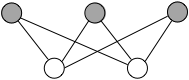
\includegraphics[scale=0.4]{FiguresGraph/outerplanarK3,2init}
        \caption{$K_{3,2}$ with its two types of vertices that are not connected two by two (white and shaded).}
\end{center}
\end{figure}
\medskip

\noindent \textit{The solution.}

We recall that a graph is outerplanar if there exists a representation where its vertices are distributed along a circle 
and no edges are crossing each other.

The solution is a case by case analysis according to all the possibilities to distribute the vertices on a circle.
\begin{figure}[h]
\begin{center}
        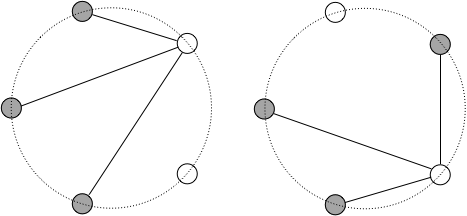
\includegraphics[scale=0.4]{FiguresGraph/outerplanarK3,2}
        \caption{The two possibilities to distribute the white and shaded vertices along a circle.}
\end{center}
\end{figure}

\medskip

\noindent \textit{Lesson learned.}


%%%
\subsection{Outerplanar graphs}

\noindent \textit{The aim.}

\medskip

\noindent \textit{The problem.}
Show that every outerplanar graph is a subgraph of a Hamiltonian graph.
\medskip

\noindent \textit{The solution.}

\medskip

\noindent \textit{Lesson learned.}



%%%
\subsection{Spanning Trees}
\label{Exercice:spanningTrees}

{\Denis I don't think it is mandatory to have such an exercice, the objective is not clear for me...}

Recall here the problem
\medskip

There are mainly two ways for constructing such a MST, each one
emphasizes a different propriety of the MST, namely, avoid cycles and
minimize the span.  In both cases, the edges are sorted in increasing
order of weights.  More precisely, the first one constructs a subtree
which partially spans the graph by adding at each step the minimum
neighboring edge while the other add successively the edges of minimal
weights that do not create a cycle.





%%%%%%%%%%%%%%%%%%%%%%%%%%%%%%%%%%%%%%%%%


\section{misc}

%
%\subsection{To include at the proper place}
%
%Prove Proposition~\ref{thm:equality=finest-equiv}
%
%{\Arny I would put put this as an exercise in SETS -- the statement of the result appears in Section~\ref{sec:equiv-relation}.}
%
%{\Denis the exercise already existed...}



\subsection{To include at the proper place}

\textbf{ Play} with negating strong (weak) relations to get weak (strong) ones.

{\Arny This refers to Eq.~(\ref{eq:NOT-rho-notation}), so it belongs near Section~\ref{sec:relation}.  The main point is to verify that the NEGATION of a weak order-like relation is a strong order-like relation, and vice versa.}
 
\subsection{To include at the proper place}

 The biggest and smallest elements of
${\cal P}(S)$ are, respectively, the set $S$ itself and the empty set
$\emptyset$.

{\Arny Power sets are first defined in Section~\ref{sec:set-concepts}.}

\subsection{To include at the proper place}

Complete the proof of Fig. xx and similar geometric arguments: show
that all points in the areas are captured
{\Denis What is this figure? The label (and the section) is wrong... }

{\Arny   This relates to one of the pictorial/geometric proofs of the value of a summation ---
6.10 or 6.13 or 6.14.

I need your help.  The problem that motivated me was that, even though it LOOKS as though an ``asymptotic" drawing is capturing all of the claimed points, that is not a proof.  We have to PROVE that all points are captured.}



\subsection{To include at the proper place}

Prove Proposition~\ref{thm:|Q|=|N|}

\noindent \textit{The problem:}
Prove $|\Q| \ = \ |\N|$.
\medskip

from Proposition~\ref{thm:|NxN|=|N|}.

{\Arny This is one of two places where proving stuff about $\N \times \N$ is much easier than proving stuff about $\Q$.

This is the first---easier---result.  We proved the clerically easier result---that $\N \times \N$ is countable.  We ask the reader to ``dirty their hands" and prove that $\Q$ is countable.

The second---harder---result is with uncountability; it is so hard that we do it.

So this should appear in NUMBERS2 near pairing functions.}



\subsection{The average length of a carry in a binary counter}

{\Arny The analysis here involves geometric sums, so this could be an exercise for SUMMATION.  Counters are discusses in NUMBERS3.  I would vote to put this in NUMBERS3.}

\noindent {\it The aim.}
\medskip

\noindent {\it The problem.}
%
You add from $1$ to $n$, in increments of $1$ using a counter of
binary (or, base-$2$) numerals.  Each time you increment the counter,
there is a {\it carry}.  These carries have varying lengths; for
instance, when $n = 32 = 100000_2$, the carry-lengths range
from $0$---whenever you increment an even integer---to $5$---when you
increment $31 = 11111_2$ to achieve $32 = 100000_2$. \\
{\em Prove that the average carry as you go from $1$ to $n$ has length $2$.}
\medskip

\noindent {\it The solution.}

\noindent
Half of the increments add $1$ to an even number, i.e., a number whose
binary numeral ends in ``$ \ldots 0$''.  These increments generate no
carry---or, equivalently, a carry of length $0$.

\noindent
One-quarter of the increments, which form half of the remaining
increments, execute a carry of length $1$, because they add $1$ to a
numeral that ends in ``$ \ldots 01$''.

\noindent
One-eighth of the increments, which form half of the remaining
increments, execute a carry of length $2$, because they add $1$ to a
numeral that ends in ``$ \ldots 011$''.

Continuing in this way, one can show that the average length of a
carry can be expressed in the form
\[ 
\frac{1}{2} \cdot 0 \ + \ \frac{1}{4} \cdot 1 \ + \ \frac{1}{8} \cdot
3 \ + \ \frac{1}{16} \cdot 4 \ + \ \cdots
\]
Using techniques that we cover in Chapter~\ref{ch:Summation}, one
verifies that this infinite series converges with the sum $2$.  \qed


